\section{Runtime Representation of Matches}
\label{section:Match}

To implement matches, two classes are defined - \texttt{Match} and \texttt{Binding}, as seen in Figure \ref{class-diagram-match-binding}.

\begin{figure}[H]
	\centering
	\makebox[\textwidth][c] { 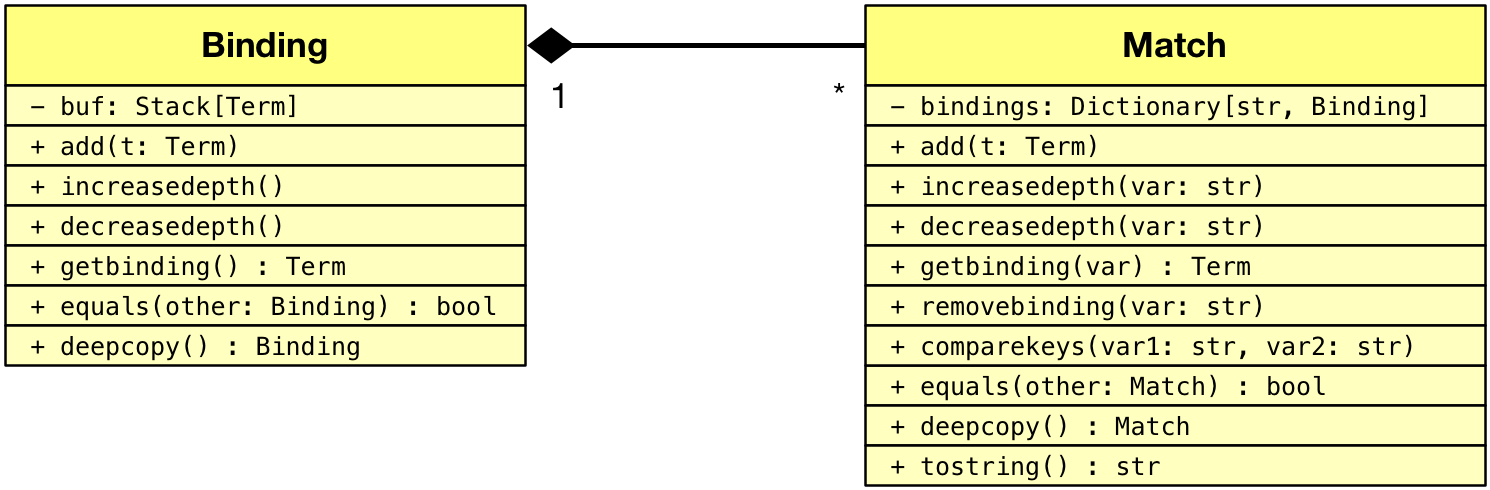
\includegraphics[scale=0.27]{class-diagram-match-binding.png} }
	\caption{\texttt{Match} and \texttt{Binding} class diagram.}
\label{class-diagram-match-binding}
\end{figure}

The \texttt{Binding} class encapsulates a stack of terms and provides three methods for its manipulation:

\begin{itemize}
\item 
\texttt{increase\_depth} pushes the term \texttt{Sequence} onto the stack provided a term on top of the stack is also a \texttt{Sequence}, otherwise it raises an Exception.

\item
\texttt{decrease\_depth} has the following behavior:
	\begin{enumerate}
		\item
        if the stack is empty, raises an Exception.
		\item
		if the stack size is 1 and the topmost element is not a \texttt{Sequence}, raises an Exception.
		\item
		if the stack size is 1 and the topmost element is a \texttt{Sequence}, does nothing.
		\item
        if the stack size is greater than one, pops the topmost \texttt{Sequence} and appends it to \texttt{Sequence} below. (this works because \texttt{increasedepth} must be called beforehand)
	\end{enumerate}

\item
\texttt{add(term)} has the following behavior:
	\begin{enumerate}
		\item
         if the stack is empty, adds \texttt{term}. 
		\item
         if the stack is not empty and the topmost term is not \texttt{Sequence}, raises an Exception
		\item
        if the stack is not empty and the topmost term is \texttt{Sequence}, adds \texttt{term} to the \texttt{Sequence}.
	\end{enumerate}
\end{itemize}

\texttt{Match} class associates pattern-variable with \texttt{Binding} instance.

\begin{itemize}
\item
\texttt{increase\_depth} calls \texttt{increase\_depth} method of relevant \texttt{Binding} instance.

\item
\texttt{decrease\_depth} calls \texttt{decrease\_depth} method of relevant \texttt{Binding} instance.

\item
\texttt{addtobinding} calls \texttt{add} method of relevant \texttt{Binding} instance with \texttt{term}.

\item
\texttt{comparekeys(key1, key2)}. Given two keys, appropriate \texttt{Binding} instances are retrieved and then the topmost terms on the stack are compared.

\item
\texttt{deepcopy} creates a new \texttt{Match} with deep-copies of \texttt{Binding} and \texttt{Term}. 
\end{itemize}
